\section {Results and Discussion}
In this section, I will provide and discuss the results of the project. I will also provide limitations and challenges.

\subsection{Finding Important Food Groups}
\flushleft \justifying I have utilized PCA to find out the important food groups in the clusters. PCA finds the importance of the food groups in the dataset for all the clusters. PCA variance and PCA Component Configurations for the cluster Age $>$ 60, and ACR $<$ 3 are given in Figure ~\ref{pca-v-food-comp}. Contributing Food Groups in the data are provided in Figure ~\ref{cluster-food-contribution}. From Figure ~\ref{pca-v-food-comp}, we see that the most important food groups for the Class: age $>$ 60, ACR $>$ 3, ACR $<$ 30 for the 1st PCA component are Total Fat, Monounsaturated Fatty Acids; Important food groups for the second PCA component are Carbohydrate, Sugar, Cholesterol (-), and Protein. 3rd PCA component shows Fibre, Sugar (-), Cholesterol (-) are important where 4th PCA component shows Protein, Total Poly Fat (-) are important. In most cases, I considered upto three or four PCA components because that can describe around 90\% of the data. From the experiment, I see that the important food groups for different clusters are very consistent with each other. It may mean that food groups taken by the population in the clusters are closely matched.

\begin{figure}
\begin{tabular}{c}
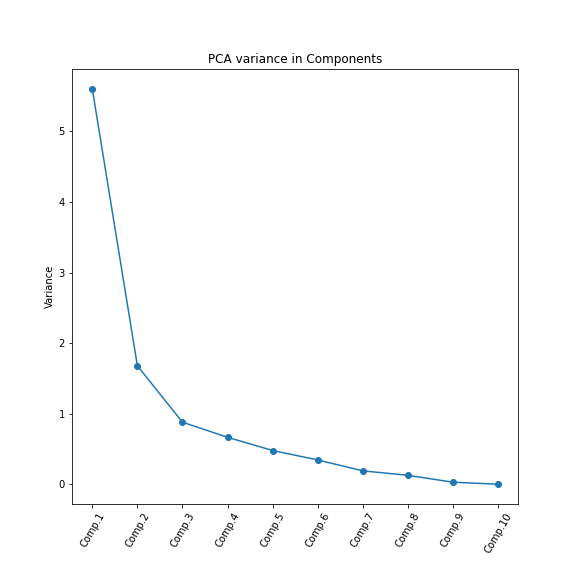
\includegraphics[scale=0.4]{images/pca_components_variance} \\
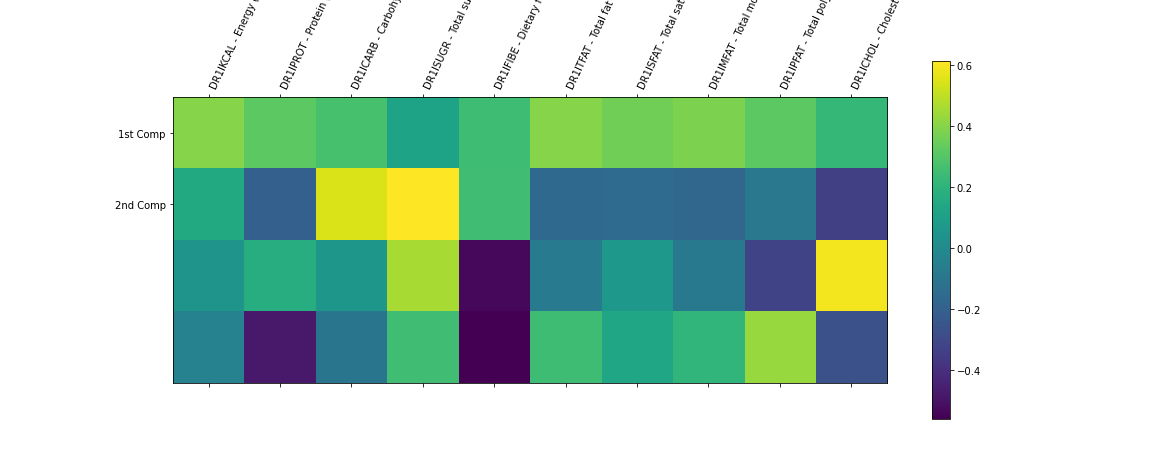
\includegraphics[scale=0.4]{images/pca_food_groups_what_contributes_to_PCA_components.png} \\
\end{tabular}
\caption{\textbf{PCA variance (top) and PCA Component Configurations for the cluster Age $>$ 60, and ACR $<$ 3 (bottom) }}
\label{pca-v-food-comp}
\vspace{0.25cm}
\end{figure}

\begin{figure}
\begin{tabular}{c}
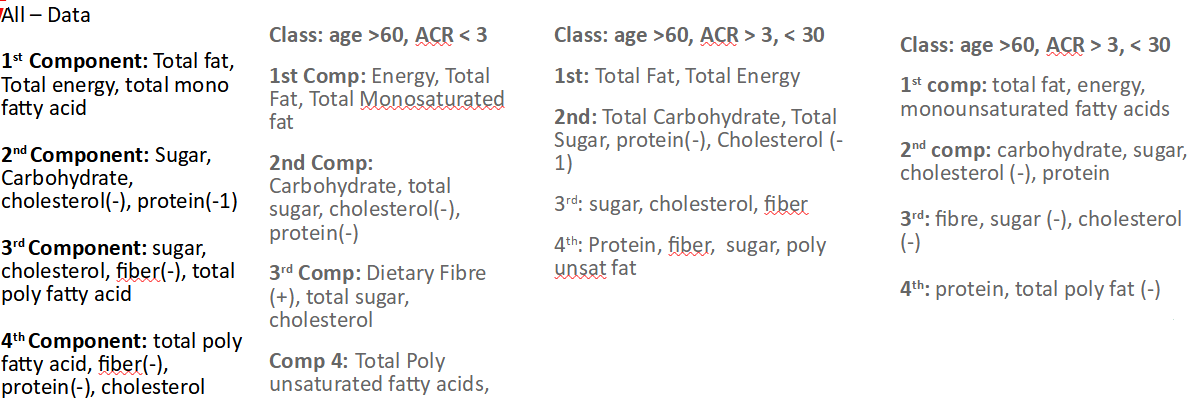
\includegraphics[scale=1]{images/important-features-food-groups.png} \\
\end{tabular}
\caption{\textbf{Contributing Food Groups in the Data Clusters}}
\label{cluster-food-contribution}
\vspace{0.25cm}
\end{figure}

\subsection{Food Group ACR Association}
Correlations between Food Groups and ACR are given in Figure ~\ref{corr-acr-food}. It also shows the correlation based on groups created on Age and ACR CKD stages. I have utilized Pearson correlation on the data after PCA. For example, Figure ~\ref{corr-acr-food} shows
that for Class 2 [Age (0, 30) ACR (3, 30)], Protein, and Fat have a correlation of -0.041 with ACR, Carbohydrate has a correlation of -0.038, and Poly unsaturated has -0.036 where Mono unsaturated has a correlation of -0.032 with ACR. For the Class 5 [Age (30, 60), ACR (3, 30)], Protein correlates -0.011, and Monounsaturated Fat correlates -0.011.


\begin{figure}
\begin{tabular}{cc}
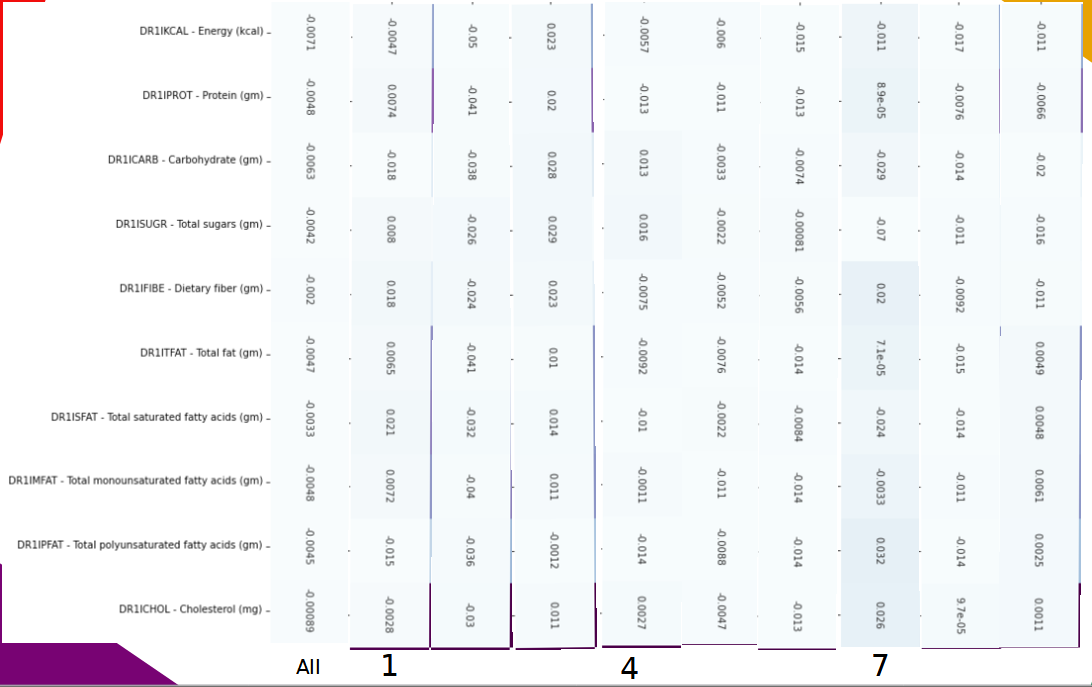
\includegraphics[scale=0.7]{images/groups-and-foods-and-correlations} \\
\end{tabular}
\caption{\textbf{Correlation of Food Groups with ACR by Age and CKD stage groups}}
\label{corr-acr-food}
\vspace{0.25cm}
\end{figure}


\begin{figure}
\begin{tabular}{c}
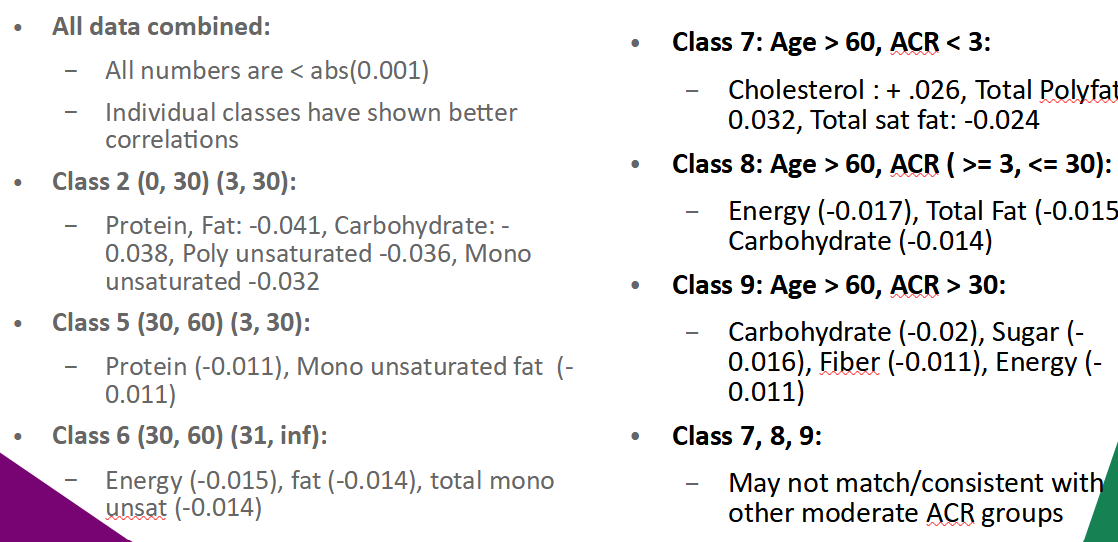
\includegraphics[scale=0.7]{images/noticeable-corr-and-food-groups.png} \\
\end{tabular}
\caption{\textbf{Some Higher Correlation numbers of Food Groups with ACR by Age and CKD stage groups}}
\label{corr-acr-food22}
\vspace{0.25cm}
\end{figure}

\subsection{Regression Coefficients}
\flushleft \justifying In this analysis, I applied regressions to find the regression coefficients i.e. to what extent a particular variable (such as the food groups) is affecting ACR. I have applied several approaches such as Linear Regression, Linear Regression with 10-Fold Cross Validation, Polynomial Regress with or without K-Fold Cross Validation, Bayesian and Random Forest regressor with or without polynomial data, and K-fold cross-validation. First, I will provide the coefficients that I found. Afterward, I will explain the significance of the coefficients. Figure ~\ref{clusters-table} provides the details of the clusters. Figure ~\ref{food-groups-abbr} shows the full form of the abbreviated food groups used in Figure ~\ref{reg-coef-food-acr}.

\flushleft \justifying Figure ~\ref{reg-coef-food-acr} shows that For Class 2 [Age(0 to 30), ACR (3 to 30) ] Higher Energy (Calorie) intake can lead to increased ACR readings. All Forms of Regression show the same. Afterward, all regression types show that Poly Unsaturated Fatty Acids have the 2nd highest contribution to ACR for Group 2. Then, all regression types show that Cholesterol has the 3rd highest contribution to ACR for Group 2. Mono Unsaturated Fatty Acids have the next level of effectiveness. Results from Linear Regression vary slightly from the other regressions I used. The code output kept at $codeoutput/regression-foodgroup-and-acr.pdf$ shows that R2 values are not significant. However, PCA data shows that Food Groups represent the data well. These may need further attention. The code $code/regression-foodgroup-and-acr.ipynb$ can be executed for any other class/cluster to find the relation of Food Groups for that Cluster. Also, the code can be applied to the Clusters created with KMeans to find relations of Food Groups with ACR. This may also show the most vulnerable groups/clusters and food groups.


\begin{figure}
\begin{tabular}{|p{4cm}|p{12cm}|}
\hline
Food Groups & Ener, Pro, Carbo, Sug, Fib, Fat, SatFatAcid, MonoUnsatFatAcid, PolyUnSatFatAcid, Choles \\
\hline
Class 2, LinearRegressionNormalizedValues & [-0.48, 0.05, 0.24, -0.15, -0.03, -0.34, 0.37, 0.17, 0.19, -0.09] \\
\hline
\hline
Class 2, LinearRegressionCrossValidation & [-0.36, -0.22, -0.05, -0.02, -0.01, -0.06, -0.01, -0.22, -0.31, -0.29] \\
\hline
Class 2, PolynomialRegressionCrossValidation & [-0.36, -0.22, -0.05, -0.02, -0.01, -0.07, -0.01, -0.23, -0.66, -0.29] \\
\hline
Class 2, BayesianPolynomialCrossValidation & [-0.36, -0.22, -0.05, -0.02, -0.01, -0.06, -0.01, -0.22, -0.31, -0.29] \\
\hline
Class 2, RandomForestRegressorCrossValidation & [-0.35, -0.21, -0.05, -0.02, -0.01, -0.06, -0.01, -0.22, -0.3, -0.28] \\
\hline
\end{tabular}
\caption{\textbf{Regression Co-Efficients of Food Groups with ACR}}
\label{reg-coef-food-acr}
\vspace{0.25cm}
\end{figure}

\begin{footnotesize}
\begin{figure}
\begin{tabular}{|p{4cm}|p{6cm}|}
\hline
Ener & Energy \\
\hline
Pro & Protein \\
Carbo & Carbohydrate \\
\hline
Sug & Sugars \\
\hline
Fib & Fiber \\
\hline
Fat & Fat \\
\hline
SatFatAcid & Saturated Fatty Acids \\
\hline
MonoUnsatFatAcid & Mono Unsaturated Fatty Acids \\
\hline
PolyUnSatFatAcid & Poly Unsaturated Fatty Acids \\
\hline
Choles & Cholesterol \\
\hline

\end{tabular}
\caption{\textbf{Food Groups: Short and Long Names}}
\label{food-groups-abbr}
\vspace{0.25cm}
\end{figure}

\end{footnotesize}

\subsection {Limitations}
\flushleft \justifying In the study, I have used the food groups found in the Dietary Intake survey. Instead, Food Groups and Sub-Groups from USDA could be used to align with USDA and other studies utilizing USDA food groups. I faced several challenges on this such as I found only 2015-2016 USDA food group data. It did not seem sufficient to assign food groups and sub-groups to the entire dataset I created. Hence, the further discovery of Data on USDA food groups will be required. I have utilized Age and ACR-Induced CKD stages for data clustering. The age group is taken from one of several approaches used for medical studies. However, a clustering algorithm such as K-Means could add value. Several CKD studies not specific to ACR utilized clustering such as Consensus/Ensembled Clustering. This study could benefit from such clustering. Additionally, I have utilized ACR as the target based on data availability. A measure such as GFR is prominently used in CKD stage determination. Hence, GFR is a better candidate than ACR to be used as the target variable. Ideally, a combination of GFR and ACR gives the true picture of CKD condition. Hence, combined ACR/GFR metric as the target variable will bring more values to the association outcome/result. Also, mortality and survival could be target variables as the first step or as the 2nd step target variable. If 2nd step ACR/GFR association can be used as the input.

\flushleft \justifying I have implemented K-Means clustering of the dataset to create 10 clusters. The cluster data can be found on GitHub under $cas-764-food-group-acr-cluster/ code/ nhanes\_output\_data \\ /classifiedGroups/ kmeanscluster$. The analysis that I have done with the initial clustered data, the same can be done with the K-Means clustered data. I could do PCA Analysis, Pearson Correlation, and all the regressions that I did (Bayesian, RandomForst, Regression with Cross Validation). Further, I could change the features to center the cluster around. These analyses could further bring clarity to the association between Food groups and ACR, and subsequently to Mortality and Survival.

\flushleft \justifying  Also, an extensive data exploration could be done at the beginning to see how the data fits into the study. A study could be R Square analysis. In my regression analysis, R Square is used; however, it could be done on a large scale at the start and then data adjustment leading to a significant R square number for the entire dataset and the clusters could make the study more valuable. Also, a pair-wise correlation study could filter out correlated features and food groups.

\section{Applications}
\flushleft \justifying The approach taken in this study can be utilized in a generic way where we want to find relations associations of some input variables to a target variable. For example, I have studied the association of Food Groups with ACR. With relevant datasets, the association of Food Groups with ACR/GFR can be discovered as well. Additionally, the regression coefficients that I am trying to find out, the same approach can be utilized in many fields such as finance, and surveillance. For example, in a target tracking application in a cluttered environment, the environmental features, as well as performance metrics, can be studied to find out how these affect the accuracy. Based, on this the algorithm could dynamically adapt to make the target tracking more accurate.


